\subsection{Connecting the Cameras} \label{connecting_the_cameras}
The cameras used in the Grimace Box need to be powered using power over Ethernet (PoE).  
To power the Ethernet connections, the cameras need to be connected to the PC through an Ethernet switch.

\begin{figure}[H]
\centering
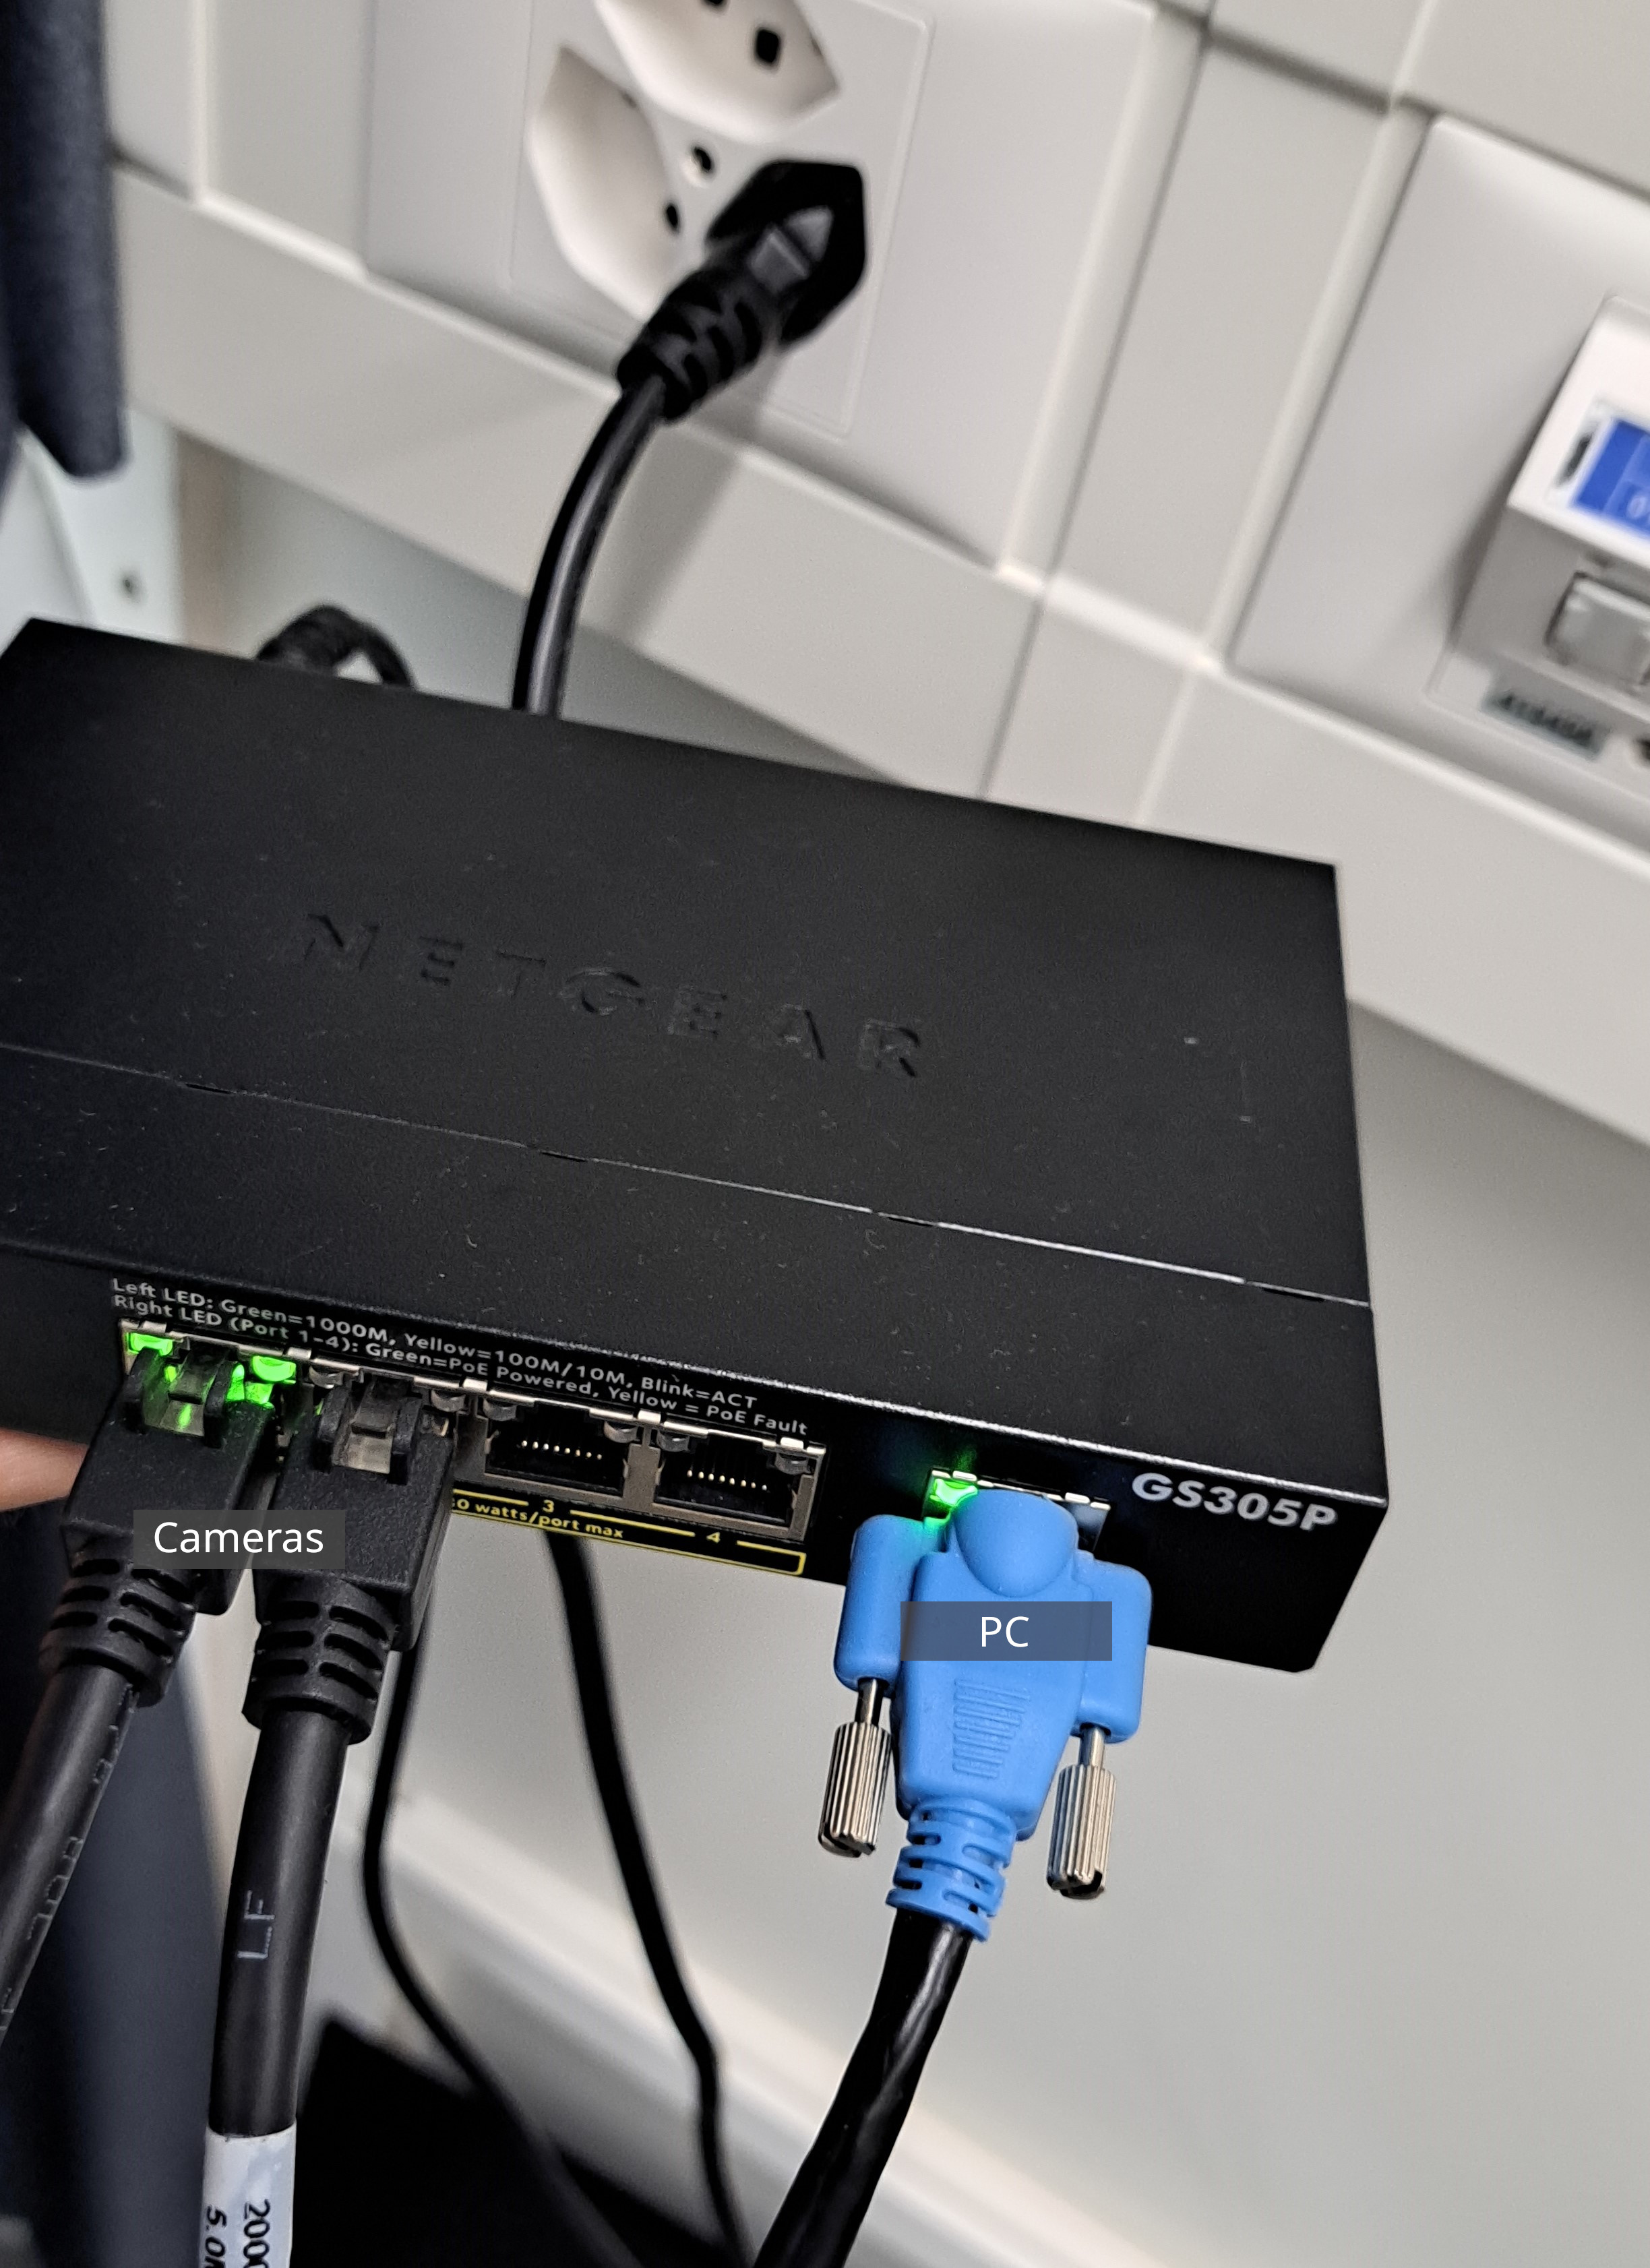
\includegraphics[width=0.65\textwidth]{content/img/ethernet_switch_setup.jpg}
\caption{\label{fig:ethernet_switch_setup}Example of an Ethernet switch with two cameras plugged in}
\end{figure}

Plug the Ethernet cables of the cameras into the free ports of the switch.\\
Connect the outgoing port of the switch to the PC.\\
Plug the switch into the power outlet.
(See \hyperref[fig:ethernet_switch_setup]{Figure} \ref{fig:ethernet_switch_setup})

\subsection{Starting the Application}
TODO: depends on how it's deployed

\subsection{Configuring the Cameras}
The cameras need to be configured before starting the recording.
Click on: \[Recording \rightarrow Configure\ Cameras \rightarrow Top\ Camera\] to open the configuration window 
for the top camera of the Grimace Box.  
From the dropdown menu, select the camera device that corresponds to the top camera.
If you are not sure which device corresponds to the top camera, select the first device.
You can later see a preview of the camera feed to verify if the correct camera is selected.  
Click on the button with the 3 dots to select a file with the configuration for the top camera.  
This file should be TODO: add info about the camera configuration file  
Configure the fps (frames per second) of the camera. The default value is 30 fps and should usually not be changed.  
Click apply to save the configuration.  
You can now see a preview of the camera feed and change the camera device if you selected the wrong one.

Repeat the same steps for the front camera by clicking on: \[Recording \rightarrow Configure\ Cameras \rightarrow Front\ Camera\].

\subsection{Configuring the Recording}
To configure settings for the recording like the recording duration and the codec used to encode the video files,
click on: \[Recording \rightarrow Configure\ Recording\].  
In the dropdown, you can either select "Manual" or "Timed", depending on whether or not you want 
the recording to stop automatically after a certain time.  
If you select "Timed", you can enter the duration of the recording in the time selector.  
You can also select the codec used to encode the video files. The default codec is FMP4. 
Alternatively FFV1 can be used to get lossless video files. However, the file size will be MUCH larger.
Click apply to save the configuration.

\subsection{Configuring the Output Files}
To configure the names and locations of the output files, click on: \[Recording \rightarrow Configure\ Files\]
You can select the folder where the video files will be saved by clicking on the button with the 3 dots.  
From the dropdown menu, you can select the naming scheme for the video files.  
If you select "Recording Number", the video files will be named \[\verb!"top_1.avi" and "front_1.avi"!\] for the first recording.  
The recording number will be increased by 1 for each new recording.  

If you select "Start Time", the video files will be named \[\verb!top_YYYYMMDDHHMMSS.avi and front_YYYYMMDDHHMMSS.avi!\] 
with \verb!YYYY! being the year, \verb!MM! the month, \verb!DD! the day, \verb!HH! the hour, \verb!MM! the minute, and \verb!SS! the second when the recording was started. \[\verb!Example: top_20240722112452.avi!\]

Alternatively, you can select "Custom Template" and enter a custom template for each of the files. 
In the custom templates, you can use the placeholders \verb!{recording_number}! and \verb!{start_time}!
to insert the recording number and start time into the file name. \[\verb!Example: my_custom_top_file_{recording_number}.avi!\]

It is advised to use a new, empty folder as the target directory.  
If the target directory already contains files with the selected naming scheme the recording number will be 
increased up to the first free number.  

Example:\\
If the target directory contains the files \path{top_1.avi} and \path{front_2.avi} and \path{top_4.avi}, 
the recording number of the next recording will be set to 3. Then the recording after that will be 5, 
as a file for recording 4 already exists.  

So unless you are continuing a previous recording session, 
use an empty folder to avoid making a mess of your file names.

\subsection{Configuring the Grimace Analysis}
To enable real-time mouse grimace scale analysis during the recording, 
click on: \[Analysis \rightarrow Configure\ Grimace\ Analysis\] 
You can enable or disable the grimace analysis by checking or unchecking the checkbox.  
If the grimace analysis is enabled, you can select the model version used for the analysis from the dropdown menu.  
The model consists of three separate machine learning models.  
You can select the device (CPU or GPU) used to run each model.
It is advised to use the GPU (Usually starting with "GeForce") if available, for all 3 models.  
You can also select how many frames of the video are sampled for the grimace analysis by configuring the "Interval Length".
If you select "1 Minute", one frame will be analyzed per minute of video. 
For each interval of 1 minute, the frame with the highest quality will be selected.  
It is advised to use the standard setting of "1 Minute".

\subsection{Saving the Configuration}
To save the current configuration, click on \[File \rightarrow Save\ Project\]
The first time you save the project, you will be asked to select a file location and name for the project file.  
Alternatively, you can click on \[File \rightarrow Save\ Project\ As\] to save the project under a different name or location.

\subsection{Loading a Configuration}
To load a previously saved configuration, click on \[File \rightarrow Load\ Project\]
This will open a file dialog where you can select the project file you want to load.

\subsection{Starting the Recording}
Once you have configured the cameras, the recording, the output files, and the grimace analysis, 
the status bar at the bottom of the main window should show "Ready to Record".
You can start the recording by clicking on the "Start Recording" button in the main window.
The status bar will change to "Recording..." and the timer in the bottom right corner will start counting up.  
If the grimace analysis is enabled, you will see the grimace scale analysis results in the grimace analysis window.  
If you have closed the grimace analysis window, 
you can open it again by clicking on \[Analysis \rightarrow Open\ Grimace\ Results\ Window\]

\subsection{Stopping the Recording}
If you have enabled timed recording, the recording will stop automatically after the configured duration.
You can stop the recording at any time by clicking on the "Stop Recording" button in the main window. 
However, if you have enabled timed recording, you will be asked for confirmation before stopping the recording early.

\subsection{Viewing the Results}
After the recording has finished, you can find the video files in the folder you configured in the output files settings.  
If you have selected the standard codec, you can open the video files with any video player like VLC or Windows Media Player.
If you have selected the FFV1 codec, you will need to use a video player that supports this codec like VLC.  
Along with each video file, a CSV file containing the frame number and timestamp of each frame in the video is generated. 
The CSV file has the same name as the video file but with the extension ".csv".
If you have enabled grimace analysis, the grimace analysis results are saved in a separate CSV file.